\section{Results on general-purpose code in full}
\label{sec:results}
The claims this paper defends, each with its interval and its label, are listed in
\texttt{CLAIMS.md}. A claim enters that file only after its report has passed an independent
review by a model from a different vendor with access to the raw records, and every section below
draws only on such reports. Section~\ref{sec:inreview} reports eight studies whose reviews took
between three and eleven rounds each to reach that point, and states what each does and does not
license. The headline results of \S\ref{sec:repeat}--\S\ref{sec:residual} come from the ceiling
study; where they cite a study from \S\ref{sec:inreview}, they say so.

Rates carry the 95\% problem-cluster percentile bootstrap as the primary interval, with the
Wilson interval beside it where the source report gives one, because problems recur across
generation batches and an interval that treats instances as independent is too narrow. For single
rates, simulations of an analogous interval under this clustered design (\S\ref{sec:stats})
suggest coverage near nominal at the headlines' rates and possible undercoverage below a true rate
of about $0.10$, under an assumed within-problem correlation. They do not measure the coverage of
the intervals reported here, and the paired contrasts and category-conditioned shares have no
measured coverage.

Sixteen comparisons were computed in the study that carries the primary contrasts, under one
Bonferroni family with a threshold of $0.00313$. That correction is applied to $p$ values and
never to intervals. Every interval in this paper is an unadjusted 95\% interval, so a directed
statement resting on an interval alone, with no $p$ value that clears its family, is worded as a
direction rather than as a finding. Each $p$ value belongs to the family of the study that computed
it. Those in \S\ref{sec:rulebook} are members of that sixteen-member family. The one in
\S\ref{sec:auditor} is the auditor-family study's single registered primary, which had no family to correct
within; it would also clear $0.00313$. The clarification study's are reported beside a primary
registered on its interval, and no correction was registered for them. Where a $p$ value appears
below, the exact McNemar value and the cluster-level sign-flip permutation value are both given,
because instances within a problem are not independent and only the second respects that.


Table~\ref{tab:primary} (Section~\ref{sec:ceiling}) collects selected primary quantities with their populations and labels;
the prose gives each one where it is used.

\subsection{Returns to repeated reading diminish short of complete}
\label{sec:repeat}

The shipped cross-vendor auditor reads an increment holistically and returns findings; an
increment is blocked if any finding is graded BLOCKER. Over eight independent readings of the same
110 defective instances, union recall rises from 10.7\% at one reading to 30.0\% [20.0, 40.7] at
eight (Figure~\ref{fig:saturation}). The eighth reading still adds 1.93 points, cluster [1.14,
2.78], against the flattening bar of 1.0 points registered before the first model call, so the bar
was not met. Under exact subset averaging that statistic has a closed form: the number of
instances flagged by exactly one of the $K$ readings divided by $K n$, here $17/(8\cdot110)$. It
is a count of singletons, not a fitted slope. Its interval resamples problems and so carries
task-sampling variance, while the statistic itself is made of reading-sampling variance, which the
interval does not describe; the bar should be read as a statement about these 17 instances rather
than about a population slope.

The constrained fit puts the asymptote at 31.5\%, but on our own registered criterion that figure
is an extrapolation, and the raw union at eight readings is the number to quote. What the data
support is diminishing returns at the budget we could afford, not saturation: at 1.9 points per
reading the curve was still climbing when we stopped. The bar also depends on where a family was
stopped. Exact subset-averaged increments do not grow with $K$ (this curve's is 2.9 points at the
fourth reading and 1.9 at the eighth), so a fixed bar is harder to meet at $K = 4$ than at
$K = 8$, and meeting it at either says little by itself about where the curve ends.

Twenty readings pooled across three auditor families reach 48.2\% [36.7, 60.0], and the same
twenty readings flag 54 of 150 correct increments, 36.0\% [28.2, 44.2]. That is more than
twice the shipped route's 16.0\%, so pooling buys its coverage at its own price. Those twenty
readings are also not twenty opportunities. The pool is eight cross-vendor, eight same-vendor and
four \texttt{astra} readings, and the same-vendor route gains 1.8 points from its first reading to
its eighth against the cross-vendor route's 19.3. It is sent temperature $0$ and returns nearly the
same verdict each time, though this design cannot say how much of that is the temperature and how
much the model. Counting that route as roughly one reading puts the depth nearer thirteen than
twenty (a heuristic, not an estimate), and the pooled figure should be read as a union over three
routes rather than over twenty independent looks.

The price is measured on the same footing. Union false positives on 150 correct increments reach
16.0\% [10.1, 22.3] at eight readings. The recall bought per point of false positive, meaning
recall gained over one reading divided by false positives gained over one reading, is
1.68 at eight, and it changes little as readings accumulate: from $K=2$ to $K=8$ the
ratio runs 1.67, 1.63, 1.64, 1.65, 1.66, 1.67, 1.68. It falls once, at $K=3$, and then rises, so repeated
reading on this route buys recall at a slightly improving price. The ratio is a quotient of two
measured rates and carries no interval of its own.



\subsection{Which model reads, and under which severity rule}
\label{sec:auditor}

Replacing the auditor with a stronger model of the generator's own vendor moved union recall at
eight readings by $-26.4$ points, cluster $[-37.3, -15.6]$: 4 of 110 against 33 of 110. Three
instances were flagged only by the new family and thirty-two only by the shipped auditor, at an
exact McNemar $p$ of $4.2 \times 10^{-7}$ and a cluster sign-flip $p$ of $2.0 \times 10^{-5}$.
This was the auditor-family study's single preregistered primary, so no family correction applies. Three
measurements qualify what it means, and none of them favours reading it as a statement about
auditing ability.

First, the two auditors are not at the same operating point, and this paper elsewhere warns against
comparing auditors at different operating points. The stronger model flags correct code at 3.3\%, or 5 of 150, which
\S\ref{sec:stats} says to quote as a count; its bootstrap interval, [0.7, 6.7], sits in the
range where simulations of an analogous interval cover about $0.89$ at a true rate of $0.03$
rather than $0.95$, so it may be narrower than it claims. The shipped auditor flags 16.0\% [10.1,
22.3]. The stronger model blocks less of everything.

Second, the sign reverses under a weaker severity rule (Figure~\ref{fig:sweep}). Counting any
finding rather than only findings graded BLOCKER, an exploratory rule that was not preregistered,
the stronger model reaches 59.1\% [47.3, 70.6] on the defect population at 34.0\% [26.5, 41.7] on
correct code, against the shipped auditor's 34.5\% [23.6, 45.5] at 19.3\% [12.8, 26.3]. The ratio
of those two rates, a derived point ratio with no interval, is 1.74 and 1.79 respectively, so
nothing here shows one family buying more recall per false positive than the other. Under
any-finding grading the stronger model's findings cover more instances, and under the BLOCKER rule
fewer, so the $-26.4$ depends on the counting rule. That does not show why the families' findings
differ, or that any finding identifies the hidden failure.

Third, the two families are not sampled alike. The shipped cross-vendor route's capability card
does not permit a temperature, so no sampling parameter is sent and the route varies between
readings; the same-vendor route permits one, the layer sends temperature $0$, and that route is
nearly deterministic. A union over nearly identical readings cannot grow much, and it does not:
over $K = 1$ to $8$ the cross-vendor family gains 19.3 points and the stronger same-vendor family gains
3.0. At one reading the gap between them is $-10.1$ points, not $-26.4$. The rest accumulates as
the two unions grow at different rates, and because model and sampling differ together, the
design cannot say how much of that difference is the sampling and how much the model. We regard
this as the most serious limitation of the contrast, and \S\ref{sec:limits} records what would be
needed to remove it.

A third family points the other way and belongs beside the headline. A high-reasoning model of the
cross-vendor family reaches 32.7\% [20.7, 45.0] union recall at four readings while flagging
10.7\% [5.9, 16.1] of correct code, against the shipped auditor's 30.0\% at 16.0\% with eight.
Paired on the same instances, the two advantages are never established together. At a common four
readings it leads on recall, $+11.5$ [2.9, 21.3], with an unresolved false-positive difference
of $-0.3$ $[-3.8, +3.4]$; against the shipped auditor's full eight it leads on false positives,
$-5.3$ $[-10.3, -0.7]$ unadjusted, but not on recall, $+2.7$ $[-6.5, +13.0]$
(\S\ref{sec:inreview}). The evidence therefore does not support ``a stronger model is a worse
auditor''. It supports the narrower statement that this particular same-vendor model, at this
the preregistered BLOCKER rule and sampled at temperature $0$, blocks far less.

A same-vendor route of the generator's own size reached lower union recall than the
cross-vendor one on these instances, $-12.7$ points $[-25.0, -0.9]$ at eight readings, signed so
that a negative value favours the cross-vendor route. The interval is unadjusted, its upper end is
0.9 points from zero, and that route is sent temperature $0$, so this is a direction under this
sampling and not a ranking of auditors. A study on a second substrate was meant to test whether the
sign reverses there; it closed without a quotable number, and on its clean run the same contrast
included zero, so no reversal was established either (\S\ref{sec:inreview}). The figure above is
a measurement on this substrate, and whether it is a property of same-vendor auditing is open.


\begin{figure}[t]
\centering
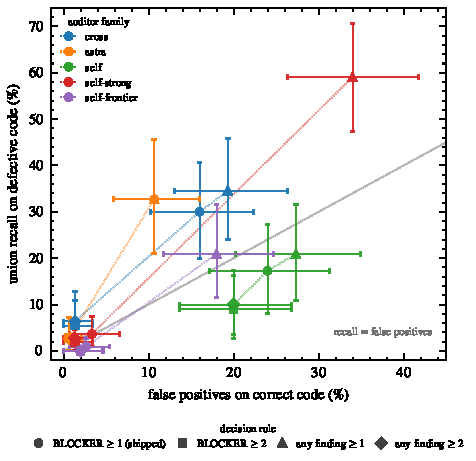
\includegraphics[width=0.46\textwidth]{fig2_sweep}
\caption{\textbf{Union recall is a property of the decision rule, not only of the auditor.}
Each point is one auditor family re-graded under one of four decision rules on the same archived
readings, with problem-cluster 95\% intervals on both axes; no new model calls were made. The
families are read at different depths: \texttt{cross}, \texttt{self} and \texttt{self-strong} at
all eight of their readings, \texttt{astra} and \texttt{self-frontier} at their four. The figure
therefore places each family at its full archived depth and is not an equal-depth comparison; the
common-depth contrasts are in Table~\ref{tab:primary}. The dotted guides join a family's four
points and are not a measured curve. Two things Table~\ref{tab:primary} cannot show: the families
do not lie on one frontier, and \texttt{self-strong} has no point under the four deterministic
rules between 3.3\% and 34.0\% false positives, exactly where a comparison matched to the
cross-vendor auditor would sit, so its ranking there is bracketed rather than measured. Nothing in
this figure assesses finding content; a flag is not a diagnosis.}
\label{fig:sweep}
\end{figure}

\subsection{One rulebook sentence moves flags, and does not measurably move outcomes}
\label{sec:rulebook}

Adding a single rule to the auditor's constitution, telling it to find what the visible tests do
not cover, moved flags on the defect population from 10 of 56 to 25 of 56: $+26.8$ points, cluster
[13.6, 40.4], exact McNemar $p = 0.0003$, cluster sign-flip $p = 0.0009$. Together with the pooled
defect-and-correct flag contrast, this is one of only two comparisons that clear the Bonferroni
threshold, and the two are the same effect seen twice.

The estimand is narrower than that of the sections above and must be read at its own scale. It is measured
on 56 instances from 41 problems, not the 110-instance defect population. It is recall at a single
reading, union recall at $K = 1$ on that population, because every loop arm revises once. And it
is exploratory, because the preregistration named outcome contrasts rather than flag contrasts. For
those reasons we do not compare its magnitude with the $-26.4$ or the $+19.3$ of the preceding
sections, which are union-recall differences at $K=8$ over 110 instances (a contrast between
routes and a gain from $K=1$).

Two costs travel with it. On correct code the same rule moved flags by $+12.50$ points. Every
discordant pair points the same way (7 against 0), so by the rule stated in \S\ref{sec:stats} the
percentile bootstrap's bound at zero is an artefact, and the admissible interval is the
unconditional one. That interval, computed with a grid-approximated nuisance supremum and ignoring
clustering, is approximate rather than guaranteed exact; it is $[-3.6, +26.8]$ and
does not exclude zero, and its exact McNemar and cluster sign-flip $p$ are both $0.0156$,
against that study's Bonferroni threshold of $0.00313$. The directed statement the records
support is the pooled one, where 23 discordant pairs point one way and 1 the other (exact McNemar
$p = 3.0\times10^{-6}$, cluster sign-flip $p = 1.0\times10^{-5}$): the sentence makes the auditor
louder overall. On the correct stratum alone the cost is $+12.50$ points with an interval that
contains zero.

The second cost is to outcomes. On the contrast that isolates the rule, the arm with the added rule against
the cross-vendor arm on hidden-suite pass rate after one revision (both strata, 112 instances on
96 problems), the effect is $+5.36$ points, cluster $[-0.89, +12.07]$, exact McNemar $p = 0.146$
and cluster sign-flip $p = 0.183$, which does not exclude zero. The rule demonstrably moves what
the auditor writes down. Whether that converts into code that passes the hidden suite is not
established, and since this paper argues that a flag is not a catch, that distinction applies to
our own intervention first.


\subsection{Most of what the auditor missed is failure the specification never determined}
\label{sec:residual}

Fifty-seven of the 110 defective instances were flagged by no reading of the three families read
at that point. That is a statement about twenty readings, not about detectability. If an instance
is caught with probability $p$ on each independent reading, twenty readings miss it with
probability $(1-p)^{20}$, which is still $98\%$ at $p = 0.001$ and $36\%$ at $p = 0.05$. Never
flagged here does not mean never flaggable, and we use the residual as a population to
characterise rather than as a set of defects shown to be invisible.

We can put a number on how flaggable it is. Reading six families at forty readings, including the
same auditor under a rulebook with one sentence added, shrinks the never-flagged set from 57 to
32 of 110, and 43 of the 68 instances both raters call specification-undetermined
are flagged by some reading of some family. Being undetermined is not sufficient for being
missed. What does not move is the composition: the undetermined share of the never-flagged set is
44 of 57, $77.2\%$, at three families and twenty readings, and 25 of 32,
$78.1\%$, at six families and forty readings.

The first classification of that residual asked whether the visible tests exercised the failing
input before it asked anything else, and it called 46 of 57 unexercised edges. Re-rating the same
instances under a second protocol reverses that. The second protocol asks first whether the
specification's prose determines the hidden suite's expected value, redefines the categories by
entailment, and uses two raters in consensus; ordering, definitions and raters all changed
together, and the study cannot isolate which mattered. The two raters agree that 44 of 57
(77.2\%, cluster [62.1, 91.1]) are cases where the prose does not settle the value, and that 2 of
57 are cases where it does and the visible tests merely never built the input. The preregistered
condition for withdrawing ``the residual is mostly unexercised edge'' fires on both of its
clauses, and that claim is withdrawn. The interval is conditional on a category and has no
committed coverage simulation, so it is uncalibrated, as is every category-conditioned interval we
report.

A classification that reverses when its protocol changes is, by itself, weak evidence about the
auditor, and the raters are not independent of it: one was the agent that ran this programme
(\S\ref{sec:methods-review}), which wrote the rubric and knew the earlier labels and which claim
was at stake. Three things support the second reading. The rubric was fixed before any label was
written. The labels were committed before we looked for outside evidence. And when a first pass
was found to have carried instance identifiers and a sheet name into the raters' view, the
labelling was re-run with identities stripped and the result held. Where an outside party had
independently recorded that one of these specifications is defective, in twelve MBPP tasks named
in a paper written for another purpose \citep{richter2026collapse}, our raters agree on 9 of the 11 that fall inside our
defect population, with both disagreements on the boundary that paper's own ``incomplete''
category draws. That check is one-sided by construction: it can support agreement where an
outsider looked, and can bound nothing about the rate.

\textbf{A rater outside the residual's families, asked a different question.} One of the two
raters above is \texttt{gpt-6-astra}, whose own misses help define the residual. A model that is
not one of the families defining it, \texttt{gpt-5.6-luna} (which read these instances only as a
secondary audit route in an earlier architecture study), later rated the same 57 instances post
hoc under a different rubric: whether the prose determines an answer at all, on a sheet showing at
most three failing inputs and never the expected values (\S\ref{sec:inreview}). It labels
38 of 57 undetermined, 13 determined and 6 cannot-tell. The two figures measure different
constructs. The earlier category also admits prose that determines an answer the oracle
contradicts, which this rubric does not count as undetermined, so 38 is not a corrected estimate
of 44. What they share is that a participating and a non-participating rater both put a majority
of the residual on the undetermined side, and the second agreed with itself on only 7 of 11
repeated items.


\begin{figure*}[t]
\centering
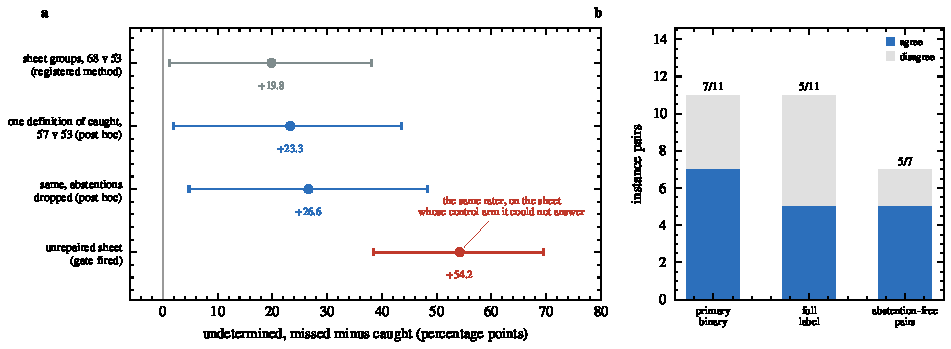
\includegraphics[width=0.94\textwidth]{fig3_residual}
\caption{\textbf{The residual contrast, printed beside the instrument that produced it.}
a, The share of instances a rater judged specification-undetermined, missed group minus
caught group, under each reading, with problem-cluster 95\% intervals. The two sheet groups use
different definitions of \emph{caught} and share eleven instances, so the two readings that apply
one definition are the ones that compare populations; both are post hoc. The red point is the same
rater on the same sheet before its control arm was rebuilt, when 42 of 53 caught entries carried
no failing-input evidence and all 42 drew \texttt{cannot-tell}. With that arm the contrast was
larger and pointed the way the hypothesis points. The repair and a fresh model run changed
together, so presentation, sampling and batch context are not separated, and a preregistered
one-third \texttt{cannot-tell} gate excluded the earlier figure. b, The same rater's agreement with itself on
the eleven instances the sheet carries twice, with identical text and identical evidence. The
contrast in a is read off the instrument in b, and the claim this paper draws
from it is stated under that constraint.}
\label{fig:residual}
\end{figure*}

\subsection{Nine further studies, and what they license}
\label{sec:inreview}

Eight further studies cleared independent review after between three and eleven rounds each, and a
ninth, on a second substrate, closed without a quotable number. We
report them here rather than folding them into the sections above because several are narrow or
negative results whose limits are part of the claim, and because the shape of their refusals is
itself a finding about this method.

\textbf{A rulebook sentence moves a second vendor's family.} The referent rule, \emph{find what the
visible tests do not cover}, raises union BLOCKER recall on \texttt{self-strong} (\texttt{claude-sonnet-4-6})
at four readings by +20.9 points, cluster [10.8, 31.8], at a false-positive cost on
correct code of +8.0 points [3.4, 12.7]. A second intervention, a rule on how findings are graded, shows no demonstrated
improvement, $+0.9$ points $[-1.8, +4.5]$, and that hypothesis fails its registered criterion,
which demonstrates neither equivalence nor that the rule did nothing. This reproduces
\S\ref{sec:rulebook}'s effect on a different vendor's model at a different $K$, with its own
price. A post hoc quantity from the same study, whether a flagged finding \emph{reports a failure}
on the instance's failing input class (says that class raises or returns the wrong value), is 3 of 110 under the shipped constitution and 27 of 110
under the rule, and it may not be quoted as defect recognition. Its rubric admits a finding even
where it grades the class non-blocking or says the specification is silent, so findings that
disclaim the requirement are counted in.

\textbf{The added rule raises union recall to 60.9\%; a higher ceiling is not established.}
On the defect population the same rule takes union recall (the identical quantity: blocked by at
least one BLOCKER, unioned over eight readings) from 33 of 110 to 67 of 110 = 60.9\%
[48.6, 72.5], +30.9 points [19.1, 43.1], at +20.7 points [12.8, 28.8] of false
positives, with a single-draw false-positive rate of 23.6\% [17.1, 30.3] that fails the product bar on all eight
draws. The caution that a flag is not a catch attaches to both figures equally. What separates
them is their price, 36.7\% [28.5, 44.8] false positives against 16.0\%, which is why the shipped
route is the shipped route. The fitted asymptotes differ by $+27.1$ points [10.9, 39.0], and
\emph{that does not establish a higher ceiling}. The cross-vendor arm never flattened, so one of
the two terms is an extrapolation. Heterogeneous low-probability detection imitates a ceiling at
this budget, since an instance found with probability $0.02$ per reading survives eight readings
about 85\% of the time. And this study's own zero-inflated estimator finds no never-detectable
class in \emph{either} arm. Its adjudication kill is arithmetic rather than a labelling artefact:
only 9 of 110 instances drew any finding on the single reading whose finding texts were archived, so the largest defect-asserting count available under
perfect adjudication was 9, below the floor of 20. Every adjudication-derived figure in it is
conditional on labels whose production can no longer be audited, because one rater's raw reply,
prompt, launcher and execution log lived only in a session scratchpad and were destroyed between
the review that flagged them and the repair.

\textbf{Corroboration does not validate a generated test.} A wrong generated test, one that fails
on the dataset's canonical solution, is not reliably recognised by asking whether further
independent generation draws also fail on the same candidate. Neither rule that makes further generation calls reaches the
preregistered threshold on the registered population, which covers failing applications on all
three candidate strata, 58 of those 107 failing applications on candidates that already fail their visible
tests. The retained wrong-test rates are 12.2\% [3.6, 22.6] (Wilson [7.0, 20.6]) for majority-over-draws
and 14.9\% [6.5, 25.5] for any-draw agreement, against a limit of 2\%, and neither is shown to improve on the free
within-draw comparator at 12.8\% [3.9, 23.9]: the better of the two rules keeps the same wrong applications plus four
correct ones, a small observed advantage the study cannot resolve. On the candidates a product
would meet, those passing their visible tests (post hoc), the rates are 6 of 33, 18.2\%
[0.0, 44.8], and 10 of 43, 23.3\% [6.8, 47.1]. The first leaves its relation to the 2\%
threshold unresolved; the second's unadjusted interval lies wholly above it, which is exploratory
evidence of exceeding it. Neither is a preregistered test on that population, whose registered
kill rule was a point estimate on the mixed population. A floor of 2.4\% holds on the original
unique-test quantity because 29 of the 45 wrong tests never fail on any candidate at all. The
claim is negative and bound to this substrate: these rules do not validate generated tests here,
which is not to say generated tests cannot be validated.

\textbf{An injected population does not give the residual result a prospective test.} We
constructed a population of injected defects intended to make specification-determinedness hold
by construction. It does not. The filter registered to recover each edit's first failing hidden
input is a truthiness check on a field the injector wrote: of 281 recorded witnesses, 179 are
strings and 102 are lists, and none is executed. Four of the remaining five filters accept cases
their registered wording excludes, such as a suite that reports success after an early exit, a
process that terminates without an assertion or an exception, and an added import from a module
already imported. No filter establishes specification entailment, and repairing the first one
alone would not have: recovering the failing input and executing a witness shows that the edit
changes behaviour on an input the hidden suite exercises, not that the specification entails the
value expected there. What may be quoted is descriptive. At eight readings the auditor blocked
90 of 92 accepted injected instances against 11 of their 92 unmodified twins,
79 discordant pairs one way and none the other, and against 33 of 110 on the natural
residual. The instances the construction's own gate \emph{refused} were blocked 31 of 40,
which is why that gate cannot be assumed conservative. A probe separates the injected set from the
natural one at 96.7\% on the items it answered, \emph{by a feature it does not identify}: the two
arms share no problem, so task composition alone could produce the result, and the probe's model
is one of the two gate models. \S\ref{sec:residual} therefore keeps exactly the status its own
study gave it, post hoc and unreplicated. A successor needs an independent party to validate the
actual violation \emph{and} the specification-entailing expected behaviour under a fixed, blinded
protocol. Neither a second substrate nor an independent rater suffices alone, because task
composition and construction confounding survive both.

\textbf{A study on a second substrate closed without a quotable number.} In a second benchmark,
the visible-test text shown to the auditor \emph{and} to the generator was sliced out of its test
class without the class header, so it failed to parse on all 300 tasks while scoring executed the
intact class. The repair for that fault introduced a second one, re-attaching a hidden method's
decorators to the first visible method on 26 tasks. A third run on a clean extraction reproduced
five of the six reversals of first-substrate findings that the second run had produced, and did not
reproduce the sixth. The
criterion registered before those numbers existed was stated over the set, so the strict reading
applies and the study is closed after three runs, about \$82, and no quotable number. Whether five
of six should have licensed the five is recorded as an open question in \texttt{CLAIMS.md}.

\textbf{Measured union recall is rule-dependent, and a headline's magnitude belongs to its own
rule.} Re-grading findings already archived by two of the studies above under four decision
rules, with no new model calls, leaves the shipped BLOCKER threshold's estimate intact for its own
rule, which \emph{was} preregistered as ``$\geq 1$ BLOCKER finding'', while \emph{reversing its
sign} under any-finding grading. That reversal is a mechanical consequence of changing what
counts, and it identifies nothing about why the families produced different findings or
different severities. At a common depth of four readings, \texttt{astra} exceeds the
cross-vendor auditor on union recall over the defect stratum by +11.5 points [2.9, 21.3], paired within instance, with a false-positive difference of $-0.3$ points
$[-3.8, +3.4]$. The two sides are not averaged alike. The cross-vendor arm has eight readings and
is averaged over all $\binom{8}{4}=70$ four-draw subsets, while \texttt{astra} has exactly four,
so $\binom{4}{4}=1$ and its estimate is a single realisation with none of its reading-selection
variance averaged out; one arm's luck in four draws is fully in the number and the other's is not.
On the cross-vendor auditor's complete eight-draw ladder the same contrast is $+2.7$ points
$[-6.5, +13.0]$ with a false-positive difference of $-5.3$ points $[-10.3, -0.7]$. That
comparison points toward lower false positives, not higher recall, on an interval whose upper end
is 0.7 points from zero and which is not adjusted for the other contrasts computed beside it, so
it is a direction the data lean and not one they establish. Observed false-positive rates near one
another are not a matched operating point, and one family has no point under the four
deterministic rules between 3.3\% and 34.0\% false positives, precisely where a matched comparison
would sit, so its ranking is bracketed rather than measured. Nothing here assesses finding content
against the hidden failure, so none of it speaks to what any finding identified.

\textbf{The ambiguity gap survives a rater that did not write the rubric, and the instrument that
shows it disagrees with itself.} The contrast in \S\ref{sec:residual} between missed and caught
instances had been rated by two models, one of them the agent that wrote the rubric. A third model
re-rated the whole sheet after we rebuilt it on mechanically recovered witnesses. That rebuild was
necessary because the control arm had been unanswerable: 42 of 53 caught entries carried no
failing-input evidence, and all 42 drew \texttt{cannot-tell}. The share labelled
\emph{undetermined} is 43 of 68 against 23 of 53, +19.8 points [1.2, 38.1]. Those two
groups are not two populations, because they define \emph{caught} differently and 11 instances
fall in both; removing those 11 from the missed group gives $+23.3$ points [2.0, 43.6], post
hoc and larger, so the overlap had understated the contrast. The limit is part of the result. On
those 11 instances, shown with identical text and identical evidence, the rater agreed
with itself on 7 of 11 on this binary outcome and 5 of 11 on the full label, where the earlier
study's two raters each agreed 11 of 11 (Figure~\ref{fig:residual}). Every interval's lower end
lies within five points of zero, and this remains a model; no human has rated this material. The
\emph{unrepaired} sheet scored $+54.2$ points [38.5, 69.5], 2.7 times the repaired contrast
and in the direction that flatters the hypothesis. That is a descriptive association between one
repair and one fresh re-rating, not evidence about specifications: the repair, the run and its
sampling changed together, and the preregistered one-third \texttt{cannot-tell} gate catches it.

\textbf{Adding the missing rule to the specification moves diagnosis, but only where the rule
matched the oracle.} The contrast above conditions on the specification; this study changes it.
The population is the 44 never-flagged instances that both earlier raters called
specification-undetermined. For the 32 on 19 problems that passed the generation gates, a model
shown the failing \emph{inputs}, but never their expected values, wrote one behavioural rule into
the prose, and an auditor re-read the same code and the same visible tests under the original, the
clarified and a same-length placebo specification, four readings each. An instance counts as
diagnosed only if both adjudicators judged some finding to state the behaviour the hidden suite
expects. Diagnosis rose from 0 of 32 to 9 of 32 under clarification and stayed at 0 of 32
under placebo. The registered primary, clarified against original, is +28.1 points,
problem-cluster 95\% interval [7.7, 51.4], which meets the registered criterion. The registered secondary, on the 23 instances where the re-rating study's consensus (\S\ref{sec:residual}) and
the third rater's label agree, is 8 of 23 against 0 of 23, $+34.8$ [10.0, 60.9].

Given the observed data, that criterion added little. Every discordant pair points one way, so no
bootstrap resample can fall below zero, and with successes on five of 19 problems a resample is
exactly zero only when it misses all five, with probability $(14/19)^{19} \approx 0.003$; the
registered run has 27 such resamples in 10{,}000. Once five success-bearing problems are observed,
the interval's exclusion of zero adds little to them (with one such problem it would not have
excluded zero), and \S\ref{sec:stats} says to read a one-signed contrast from an exact test
instead. The registration kept the bootstrap and we report it as registered, but the informative
figure is the cluster sign-flip test the registration prefers. The nine successes sit on five
problems, and the sign-flip test gives $p = 0.060$ (exactly $2/2^5 = 0.0625$ on enumeration), against $0.0039$ for
a McNemar test that counts nine independent pieces of evidence where five exist. It is not
significant at 0.05. The registered naming-rate secondary was never computed.

Two further limits are part of the result. \emph{The inferred rule contradicts the hidden suite
entirely on 23 of the 32 instances and partly on 2}, and diagnosis was 0 of 23 where it
contradicted against 9 of 9 elsewhere. That split was classified after the outcome was seen, not
assigned, and the agreeing instances may simply be the easier problems; it does not say which
property of the edits moved diagnosis. And a separate model rated the clarified prose more
determining than the original by $+28.1$ points [2.6, 54.3] but than the placebo by $+18.8$
$[-9.4, +45.2]$, so whether the placebo was inert as a specification is unresolved. One
adjudicator is the agent that ran the study and the other is \texttt{gpt-6-astra}, the model that
also reviewed this study (\S\ref{sec:methods-review}); they agreed on 84 of 91 items,
$\kappa = 0.85$, which is agreement and not accuracy. The study supports a specification-edit
contrast on these selected instances. It does not establish that underdetermination caused the
original misses, and \S\ref{sec:residual} is not strengthened into that claim by it.

\textbf{What a flag on correct code points at.} The false-positive rates above count flags on code
that passes its hidden suite. A suite may leave behaviour unexercised, so a flag there need not be
a false alarm. A preregistered study re-read the 150 correct instances with the shipped route at
eight readings, keeping the finding texts the ceiling study had discarded; 20 were flagged ($13.3\%$
[7.9, 19.2], a fresh sample of the route's $16.0\%$). A model given each finding, but not the
reference solution or the hidden tests, extracted the concrete inputs it names, and candidate and
reference were run on them. Two of the 20 disagreed with the reference on an extracted
input the hidden suite does not exercise ($10.0\%$, problem-cluster [0.0, 26.3]); on nine they
agreed, and nine yielded no valid input. Because the interval includes zero, the registered
reading is that at this resolution there is no evidence that this route's flags on test-passing
code identify reference disagreements. No class licenses the words ``true positive'' or ``false
alarm'': a disagreement does not show that the specification was violated, and agreement on an
extracted input does not show a finding wrong.

\textbf{What the refusals were about.} These eight studies cleared review at rounds 3, 3, 4, 6, 7,
9, 10 and 11, fifty-three rounds in all. Most of those rounds ended in a refusal of the
\emph{repair} rather than of the measurement. Measurements moved on review in three of the eight:
the sweep's first review found its loader reading one family's draws 4 to 8 as 1 to 5 and
another's population from a partial draw, and every cross-family figure was recomputed; a label
count in the third rating's report was 71 where its data say 67; and the clarification study's
primary moved by one instance and three classification rows (\S\ref{sec:methods-review}). Every
figure above reproduced independently at every round after its last repair. The recurring failure
was a check or a sentence that claimed more than it delivered. A binding protected one sentence of
a withdrawal spread across six; when it was rewritten to protect all six, two of them were
truncated before the words that carried their meaning. One check stripped HTML comments and called
the result what a reader sees, and one test was named for a code path that never called it. A
second pattern appeared in the last thirteen rounds: most of those refusals were
\emph{overstatements away from our own interest}, such as a registration whose chronology its own
repository contradicted, a withdrawal that overcorrected past what the record supported, a
publication prohibition a registered gate never imposed, and a limitation credited to another
study's work that the other study had not performed. Understatement was corrected as
often as overstatement; in both cases the fix was a smaller claim written where the claim was.

\subsection{What follows for a recall number}

Taken together, the results above say an audit recall figure is a joint property of the auditor
and its material. It moves with which route reads (model and sampling together, which this design
does not separate), with what the rulebook tells it to look for, and with the severity threshold
at which a finding becomes a block, which is rarely reported. What it misses is associated with
whether the hidden suite asks a question the specification answers. That association is observed
in the residual and in a specification-edit contrast on selected instances; it is not isolated as a
cause.
